\section{DIL\_\-Visualize  Class Reference}
\label{classDIL__Visualize}\index{DIL_Visualize@{DIL\_\-Visualize}}
{\tt \#include $<$dil2al.hh$>$}

Inheritance diagram for DIL\_\-Visualize::\begin{figure}[H]
\begin{center}
\leavevmode
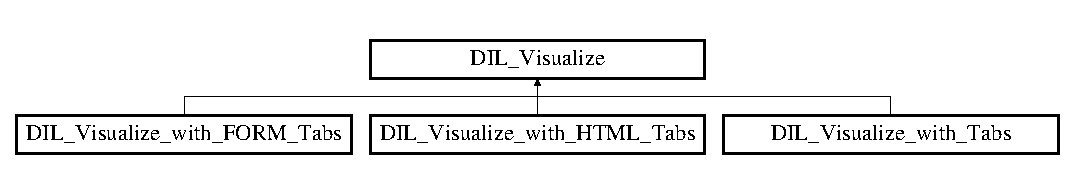
\includegraphics[height=1.83007cm]{classDIL__Visualize}
\end{center}
\end{figure}
\subsection*{Public Methods}
\begin{CompactItemize}
\item 
{\bf DIL\_\-Visualize} ({\bf DIL\_\-Hierarchy\_\-Level\_\-Data} $\ast$ld=NULL)
\item 
virtual void {\bf Initialize} ()=NULL
\item 
virtual void {\bf Attach\_\-Level\_\-Data} ({\bf DIL\_\-Hierarchy\_\-Level\_\-Data} \&ld)
\item 
virtual void {\bf Detach\_\-Level\_\-Data} ()
\item 
virtual {\bf DIL\_\-Hierarchy\_\-Level\_\-Data} $\ast$ {\bf Level\_\-Data} ()
\item 
virtual void {\bf Visualize\_\-Element} ({\bf DIL\_\-entry} $\ast$de, int depth)=NULL
\item 
virtual void {\bf Visualize\_\-Not\-Shown} (int numdependencies, int depth)=NULL
\item 
virtual {\bf String} {\bf Output} ()=NULL
\item 
virtual double {\bf get\_\-cumlikelihood} ()
\item 
virtual void {\bf set\_\-cumlikelihood} (double cumlike)
\end{CompactItemize}
\subsection*{Public Attributes}
\begin{CompactItemize}
\item 
{\bf PLLRoot}$<$ {\bf DIL\_\-Hierarchy\_\-Level\_\-Data} $>$ {\bf ldroot}
\end{CompactItemize}
\subsection*{Protected Attributes}
\begin{CompactItemize}
\item 
double {\bf cumlikelihood}
\item 
{\bf DIL\_\-Hierarchy\_\-Level\_\-Data} $\ast$ {\bf leveldata}
\end{CompactItemize}


\subsection{Constructor \& Destructor Documentation}
\index{DIL_Visualize@{DIL\_\-Visualize}!DIL_Visualize@{DIL\_\-Visualize}}
\index{DIL_Visualize@{DIL\_\-Visualize}!DIL_Visualize@{DIL\_\-Visualize}}
\subsubsection{\setlength{\rightskip}{0pt plus 5cm}DIL\_\-Visualize::DIL\_\-Visualize ({\bf DIL\_\-Hierarchy\_\-Level\_\-Data} $\ast$ {\em ld} = NULL)\hspace{0.3cm}{\tt  [inline]}}\label{classDIL__Visualize_a0}




Definition at line 745 of file dil2al.hh.

References cumlikelihood.



\footnotesize\begin{verbatim}745 : cumlikelihood(0.0), leveldata(ld) {}
\end{verbatim}\normalsize 


\subsection{Member Function Documentation}
\index{DIL_Visualize@{DIL\_\-Visualize}!Attach_Level_Data@{Attach\_\-Level\_\-Data}}
\index{Attach_Level_Data@{Attach\_\-Level\_\-Data}!DIL_Visualize@{DIL\_\-Visualize}}
\subsubsection{\setlength{\rightskip}{0pt plus 5cm}virtual void DIL\_\-Visualize::Attach\_\-Level\_\-Data ({\bf DIL\_\-Hierarchy\_\-Level\_\-Data} \& {\em ld})\hspace{0.3cm}{\tt  [inline, virtual]}}\label{classDIL__Visualize_a2}




Definition at line 750 of file dil2al.hh.

Referenced by Show\_\-DIL\_\-Hierarchy().



\footnotesize\begin{verbatim}750 { leveldata = &ld; }
\end{verbatim}\normalsize 
\index{DIL_Visualize@{DIL\_\-Visualize}!Detach_Level_Data@{Detach\_\-Level\_\-Data}}
\index{Detach_Level_Data@{Detach\_\-Level\_\-Data}!DIL_Visualize@{DIL\_\-Visualize}}
\subsubsection{\setlength{\rightskip}{0pt plus 5cm}virtual void DIL\_\-Visualize::Detach\_\-Level\_\-Data ()\hspace{0.3cm}{\tt  [inline, virtual]}}\label{classDIL__Visualize_a3}




Definition at line 751 of file dil2al.hh.

Referenced by Show\_\-DIL\_\-Hierarchy().



\footnotesize\begin{verbatim}751 { leveldata = NULL; }
\end{verbatim}\normalsize 
\index{DIL_Visualize@{DIL\_\-Visualize}!get_cumlikelihood@{get\_\-cumlikelihood}}
\index{get_cumlikelihood@{get\_\-cumlikelihood}!DIL_Visualize@{DIL\_\-Visualize}}
\subsubsection{\setlength{\rightskip}{0pt plus 5cm}virtual double DIL\_\-Visualize::get\_\-cumlikelihood ()\hspace{0.3cm}{\tt  [inline, virtual]}}\label{classDIL__Visualize_a8}




Definition at line 756 of file dil2al.hh.

References cumlikelihood.

Referenced by Show\_\-DIL\_\-Hierarchy().



\footnotesize\begin{verbatim}756 { return cumlikelihood; }
\end{verbatim}\normalsize 
\index{DIL_Visualize@{DIL\_\-Visualize}!Initialize@{Initialize}}
\index{Initialize@{Initialize}!DIL_Visualize@{DIL\_\-Visualize}}
\subsubsection{\setlength{\rightskip}{0pt plus 5cm}virtual void DIL\_\-Visualize::Initialize ()\hspace{0.3cm}{\tt  [virtual]}}\label{classDIL__Visualize_a1}




Reimplemented in {\bf DIL\_\-Visualize\_\-with\_\-Tabs} {\rm (p.\,\pageref{classDIL__Visualize__with__Tabs_a1})}, {\bf DIL\_\-Visualize\_\-with\_\-HTML\_\-Tabs} {\rm (p.\,\pageref{classDIL__Visualize__with__HTML__Tabs_a1})}, and {\bf DIL\_\-Visualize\_\-with\_\-FORM\_\-Tabs} {\rm (p.\,\pageref{classDIL__Visualize__with__FORM__Tabs_a1})}.\index{DIL_Visualize@{DIL\_\-Visualize}!Level_Data@{Level\_\-Data}}
\index{Level_Data@{Level\_\-Data}!DIL_Visualize@{DIL\_\-Visualize}}
\subsubsection{\setlength{\rightskip}{0pt plus 5cm}virtual {\bf DIL\_\-Hierarchy\_\-Level\_\-Data}$\ast$ DIL\_\-Visualize::Level\_\-Data ()\hspace{0.3cm}{\tt  [inline, virtual]}}\label{classDIL__Visualize_a4}




Definition at line 752 of file dil2al.hh.

Referenced by DIL\_\-Visualize\_\-with\_\-FORM\_\-Tabs::Visualize\_\-Element(), DIL\_\-Visualize\_\-with\_\-FORM\_\-Tabs::Visualize\_\-Not\-Shown(), and DIL\_\-Visualize\_\-with\_\-FORM\_\-Tabs::Visualize\_\-Plan\_\-Entry().



\footnotesize\begin{verbatim}752 { return leveldata;  }
\end{verbatim}\normalsize 
\index{DIL_Visualize@{DIL\_\-Visualize}!Output@{Output}}
\index{Output@{Output}!DIL_Visualize@{DIL\_\-Visualize}}
\subsubsection{\setlength{\rightskip}{0pt plus 5cm}virtual {\bf String} DIL\_\-Visualize::Output ()\hspace{0.3cm}{\tt  [virtual]}}\label{classDIL__Visualize_a7}




Reimplemented in {\bf DIL\_\-Visualize\_\-with\_\-Tabs} {\rm (p.\,\pageref{classDIL__Visualize__with__Tabs_a4})}, {\bf DIL\_\-Visualize\_\-with\_\-HTML\_\-Tabs} {\rm (p.\,\pageref{classDIL__Visualize__with__HTML__Tabs_a4})}, and {\bf DIL\_\-Visualize\_\-with\_\-FORM\_\-Tabs} {\rm (p.\,\pageref{classDIL__Visualize__with__FORM__Tabs_a4})}.\index{DIL_Visualize@{DIL\_\-Visualize}!set_cumlikelihood@{set\_\-cumlikelihood}}
\index{set_cumlikelihood@{set\_\-cumlikelihood}!DIL_Visualize@{DIL\_\-Visualize}}
\subsubsection{\setlength{\rightskip}{0pt plus 5cm}virtual void DIL\_\-Visualize::set\_\-cumlikelihood (double {\em cumlike})\hspace{0.3cm}{\tt  [inline, virtual]}}\label{classDIL__Visualize_a9}




Definition at line 757 of file dil2al.hh.

References cumlikelihood.

Referenced by Show\_\-DIL\_\-Hierarchy().



\footnotesize\begin{verbatim}757 { cumlikelihood=cumlike; }
\end{verbatim}\normalsize 
\index{DIL_Visualize@{DIL\_\-Visualize}!Visualize_Element@{Visualize\_\-Element}}
\index{Visualize_Element@{Visualize\_\-Element}!DIL_Visualize@{DIL\_\-Visualize}}
\subsubsection{\setlength{\rightskip}{0pt plus 5cm}virtual void DIL\_\-Visualize::Visualize\_\-Element ({\bf DIL\_\-entry} $\ast$ {\em de}, int {\em depth})\hspace{0.3cm}{\tt  [virtual]}}\label{classDIL__Visualize_a5}




Reimplemented in {\bf DIL\_\-Visualize\_\-with\_\-Tabs} {\rm (p.\,\pageref{classDIL__Visualize__with__Tabs_a2})}, {\bf DIL\_\-Visualize\_\-with\_\-HTML\_\-Tabs} {\rm (p.\,\pageref{classDIL__Visualize__with__HTML__Tabs_a2})}, and {\bf DIL\_\-Visualize\_\-with\_\-FORM\_\-Tabs} {\rm (p.\,\pageref{classDIL__Visualize__with__FORM__Tabs_a2})}.

Referenced by Show\_\-DIL\_\-Hierarchy().\index{DIL_Visualize@{DIL\_\-Visualize}!Visualize_NotShown@{Visualize\_\-NotShown}}
\index{Visualize_NotShown@{Visualize\_\-NotShown}!DIL_Visualize@{DIL\_\-Visualize}}
\subsubsection{\setlength{\rightskip}{0pt plus 5cm}virtual void DIL\_\-Visualize::Visualize\_\-Not\-Shown (int {\em numdependencies}, int {\em depth})\hspace{0.3cm}{\tt  [virtual]}}\label{classDIL__Visualize_a6}




Reimplemented in {\bf DIL\_\-Visualize\_\-with\_\-Tabs} {\rm (p.\,\pageref{classDIL__Visualize__with__Tabs_a3})}, {\bf DIL\_\-Visualize\_\-with\_\-HTML\_\-Tabs} {\rm (p.\,\pageref{classDIL__Visualize__with__HTML__Tabs_a3})}, and {\bf DIL\_\-Visualize\_\-with\_\-FORM\_\-Tabs} {\rm (p.\,\pageref{classDIL__Visualize__with__FORM__Tabs_a3})}.

Referenced by Show\_\-DIL\_\-Hierarchy().

\subsection{Member Data Documentation}
\index{DIL_Visualize@{DIL\_\-Visualize}!cumlikelihood@{cumlikelihood}}
\index{cumlikelihood@{cumlikelihood}!DIL_Visualize@{DIL\_\-Visualize}}
\subsubsection{\setlength{\rightskip}{0pt plus 5cm}double DIL\_\-Visualize::cumlikelihood\hspace{0.3cm}{\tt  [protected]}}\label{classDIL__Visualize_n0}




Definition at line 742 of file dil2al.hh.

Referenced by DIL\_\-Visualize(), get\_\-cumlikelihood(), set\_\-cumlikelihood(), DIL\_\-Visualize\_\-with\_\-FORM\_\-Tabs::Visualize\_\-Element(), and DIL\_\-Visualize\_\-with\_\-FORM\_\-Tabs::Visualize\_\-Plan\_\-Entry().\index{DIL_Visualize@{DIL\_\-Visualize}!ldroot@{ldroot}}
\index{ldroot@{ldroot}!DIL_Visualize@{DIL\_\-Visualize}}
\subsubsection{\setlength{\rightskip}{0pt plus 5cm}{\bf PLLRoot}$<${\bf DIL\_\-Hierarchy\_\-Level\_\-Data}$>$ DIL\_\-Visualize::ldroot}\label{classDIL__Visualize_m0}




Definition at line 748 of file dil2al.hh.

Referenced by Show\_\-DIL\_\-Hierarchy().\index{DIL_Visualize@{DIL\_\-Visualize}!leveldata@{leveldata}}
\index{leveldata@{leveldata}!DIL_Visualize@{DIL\_\-Visualize}}
\subsubsection{\setlength{\rightskip}{0pt plus 5cm}{\bf DIL\_\-Hierarchy\_\-Level\_\-Data}$\ast$ DIL\_\-Visualize::leveldata\hspace{0.3cm}{\tt  [protected]}}\label{classDIL__Visualize_n1}




Definition at line 743 of file dil2al.hh.

The documentation for this class was generated from the following file:\begin{CompactItemize}
\item 
{\bf dil2al.hh}\end{CompactItemize}
